\graphicspath{{./Lecture12/}}

\section{Wave Equations: Neumann Boundary Conditions}

Solve IBVP: $y_{tt} = a^2 y_{xx}$

Boundary conditions: $y_x(0,t) = y_x (L,t) = 0$ $\Rightarrow$ Homogeneous Neumann boundary conditions. 

\hfill

Initial conditions: $y(x,0) = f(x)$, $y_t(x,0) = 0 = g(x)$ (Therefore zero initial velocity, with specified initial displacement). 

Split into two problems (w and z). Because $g(x) = 0$, we only have the $z$ equation. For the solution, we use separation of variables. \footnote{Note that left and right side of table are entirely separate. }



$$\begin{array}{l|r}
     X'' + \lambda X = 0 & \ddot T + a^2 \lambda T = 0\\
     \Rightarrow X_n(x) = \cos \left( \frac{n \pi x}{L} \right) & \dot{T}_n (0) = 0 \\
     \lambda_n = \left( \frac{n \pi}{L} \right)^2 & T_n(t) = A_n \cos \left( \frac{n \pi a}{L}  t \right)\\
     X_0(x) = 1 \Rightarrow \lambda_0 = 0 & T_0(t) = 1 
\end{array}$$

The solution would be:

$$y(x,t) = A_0 + \sum_{n = 1}^\infty A_n \cos \left( \frac{n \pi x}{L}  \right) \cos \left( \frac{n \pi a}{L}  t \right)$$

Note that $A_0$ is the multiplication of $X_0 T_0$ terms.

$$\text{At } t = 0 \longrightarrow y(x,0) = A_0 + \sum_{n = 1}^\infty A_n \cos \left( \frac{n \pi x}{L}  \right) = f(x)$$

We construct Fourier cosine series for $f(x)$. 

$$f(x) = \frac{a_0}{2} + \sum{n=  1}^\infty a_n \cos \left( \frac{n \pi x}{L}  \right)$$

$$\Rightarrow A_0 = \frac{a_0}{2}, A_n = a_n$$

\textbf{Note: We can do a similar solution if initial velocity is given. }

\subsection{Recap}

\begin{itemize}
    \item Introduced wave equation
    \item Developed separation of variables method to find its solution
    \begin{itemize}
        \item Dirichlet and Neumann boundary conditions
        \item Examples and normal modes
    \end{itemize}
\end{itemize}

Now: New method. 

\begin{itemize}
    \item New look at the wave equation and we solve the wave equation using \textbf{D'Alembert's solution}. 
\end{itemize}

\section{D'Alembert's Solution}

$$y_{tt} = a^2 y_{xx}$$

Let's see if we can guess a solution of exponential format. 

$$y(x,t) = e^{i k x + \sigma t}$$

where $k$ and $\sigma$ are constants. \footnote{Try this guess solution with heat solution! You will find that it does work for heat equations. }

Substitute the guessed solution into the PDE. 

$$y_tt = \sigma^2 e^{i k x + \sigma t}$$

$$y_{xx} = - k^2 e^{i k x + \sigma t}$$

Now, substitute this into the PDE:

$$\left(\sigma^2 + a^2 k^2 \right) e^{i k t + \sigma t} = 0$$

$$\Rightarrow \sigma = \pm i k a$$

$$y_1 (x,t) = e^{i k (x - at)}$$

$$y_2(x,t) = e^{i k(x + at)}$$

$x \pm at$ are known as characteristics, these are lines in $x$ and $t$ along which the initial conditions (and general information) travels. 

The question here is this: Can this form of solution be more general such that we can apply it to any wave equation?

$$y_1 (x,t) = F(x-at), y_2(x,t) = G(x+at)$$

Can we find a general equation that satisfies the wave equation?


\begin{figure}[ht]
    \centering
    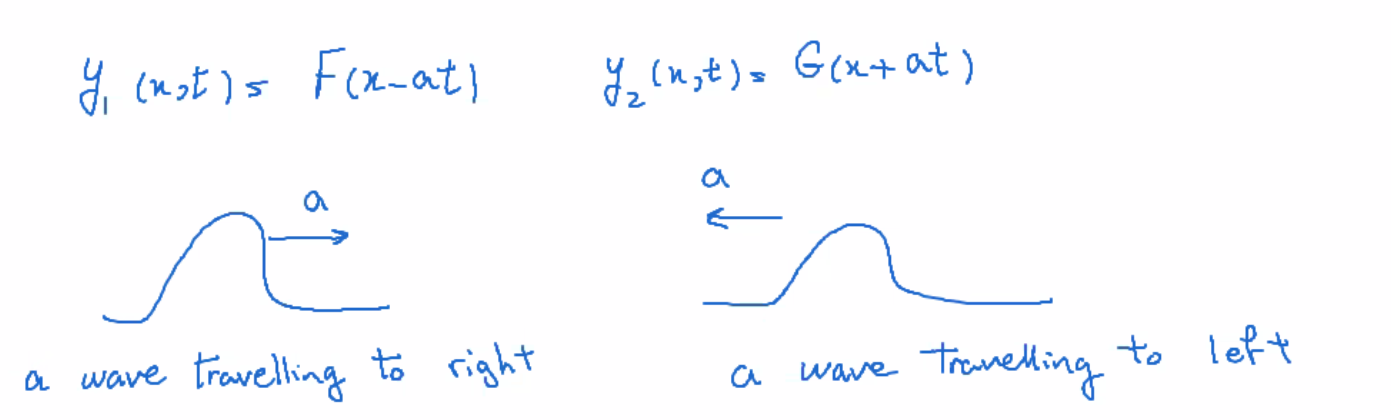
\includegraphics[width = 0.9 \textwidth]{image1.png}
    \caption{$F(x-at)$ is a wave travelling to the right with a speed of $a$. $G(x+at)$ is a wave travelling to the left with a speed of $a$. }
    \label{fig:Wave_directions}
\end{figure}

Hence, a general solution:

$$y(x,t) = F(x-at) + G(x+at)$$

Does it satisfy the PDE?

$$\begin{matrix} y(x,0) = f(x) & \Rightarrow & F(x) + G(x) = f(x) & (1)\\ y_t(x,0) = g(x) & \Rightarrow & -a F'(x) + a G'(x) = g(x) & (2) \end{matrix}$$

We get (2) from:

$$-a F(x) + a G(x) = \int_0^x g(s) ds + A$$

$$(1) xa + 2 \Rightarrow 2aG(x) + f(x) = \int_0^x g(s) ds + A$$

$$\Rightarrow G(x) = \frac{1}{2} f(x) + \frac{1}{2a} \int_0^x g(s) ds + \frac{A}{2a}$$

To find $F(x)$:

$$(1) xa - (2) \Rightarrow 2a F(x) = a f(x) - \int_0^x g(s) ds - A$$

$$\Rightarrow F(x) = \frac{1}{2} f(x) - \frac{1}{2a} \int_0^x g(s) ds - \frac{A}{2a}$$

Now, substitute these into the general solution: (plug into $y(x,t) = F(x-at) + G(x+at)$)

This gives us:

$$\frac{1}{2} f(x-at) - \frac{1}{2a} \int_0^{x-at} g(s) ds + \frac{1}{2} f(x+at) + \frac{1}{2a} \int_0^{x+at} g(s) ds$$

Note that $- \frac{A}{2a}$ and $\frac{A}{2a}$ cancel. 

\begin{equation}
    y(x,t) = \frac{1}{2} \left[ \underbrace{f(x-at)}_{\text{half of init  cond travels right}} + \underbrace{f(x+at)}_{\text{half of init cond travels left}} \right] + \frac{1}{2a} \int_{x-at}^{x+at} g(s) ds
\end{equation}

N.B. Above analysis has no boundary conditions: $-\infty < x < \infty$

\hfill

What if the problem has boundary condition?

Let $F^o (x)$ and $G^o (x)$ be the odd\footnote{ (Assumes Dirichlet boundary conditions)} 2L-periodic extension of $f(x)$ and $g(x)$ respectively:

$$y(x,t) = \frac{1}{2} \left[ F^o (x-at) + F^o (x+at) \right] + \frac{1}{2a} \int_{x-at}^{x+at} G^o (s) ds$$

Boundary conditions: \footnote{Note that we are using the properties of odd functions to cancel out both F and G. }

$$y(0,t) = \underbrace{ \frac{1}{2} \left[ F^o (-at) + F^o (at) \right]}_{=0} + \underbrace{\frac{1}{2a} \int_{-at}^{at} G^o (s) ds}_{ = 0} = 0$$

What's the relationship between D'Alembert's formula and the separation of variables?

$$y(x,t) = \sum_{n = 1}^\infty \sin \left( \frac{n \pi x}{L} \right) \left[ b_n \frac{L}{n \pi a} \sin \left( \frac{n \pi a}{L}  t\right) + b_n' \cos \left( \frac{n \pi a}{L} t \right) \right]$$

Recall trig formulae:

$$\sin(A) \sin(B) = \frac{1}{2} \left[ \cos(A-B) - \cos(A+B) \right]$$

$$\sin(A) \cos(B) = \frac{1}{2} \left[ \sin(A-B) + \sin(A+B) \right]$$

Let's apply these:

$$y(x,t) = \frac{1}{2} \sum_{n  =1}^\infty \frac{b_n L}{n \pi a} \underbrace{\left[ \cos \left( \frac{n \pi}{L} (x-at) \right) - \cos \left( \frac{n \pi}{L} (x+at) \right) \right]}_{\text{Let's write this in integral format}} \rightarrow$$

$$\hookrightarrow + b_n' \left[ \sin \left( \frac{n \pi}{L} (x-at) \right) - \sin \left( \frac{n \pi}{L} (x+at) \right) \right]$$

$$y(x,t) = \frac{1}{2} \sum_{n = 1}^\infty b_n' \left[ \sin \left( \frac{n \pi}{L} (x-at) \right) - \sin \left( \frac{n \pi}{L} (x+at) \right) \right] \rightarrow$$

$$ \hookrightarrow + \frac{1}{2a} \sum_{n = 1}^\infty b_n \int_{x - at}^{x+at} \sin \left( \frac{n \pi s}{L} \right) ds$$

Recall: 

$$\sum_{n = 1}^\infty b_n' \sin(\frac{n \pi x}{L}) = f(x)$$

and

$$\sum_{n  =1}^\infty b_n \sin \left( \frac{n \pi x}{L} \right) = g(x)$$

$\Rightarrow$ d'Alembert's solution:

$$y(x,t) = \frac{1}{2} \left[ f(x-at) + f(x+at) \right] + \frac{1}{2a} \int_{x-at}^{x+at} g(s) ds$$

Both methods give similar solution. 